%%%%%%%%%%%%%%%%%%%%%%%%%%%%%%%%%%%%%%%%%%%%%%%%%%%%%%%%%%%%%%%%%%%%%%%%
% Author  : Andrei Sobolevski (April 2009)
% License : Creative Commons attribution license
% Title   : Map of scientific interactions of researchers
%           affiliated in 2008 to the J.-V. Poncelet laboratory
%           (UMI 2615 CNRS, http://www.poncelet.ru)
% Notes   : Produced for the 2008 annual report of the lab;
%           layout of subnodes is a result of manual optimization
% Tags    : mindmap, layers
% Submitted to TeXample.net on 16 January 2010

\documentclass{article}
%%%<
\usepackage{verbatim}
%%%>
\usepackage{tikz,times}
\usepackage[paperwidth=25cm,paperheight=22cm,left=1cm,top=1cm]{geometry}

\usetikzlibrary{mindmap,backgrounds}

\pagestyle{empty}

\begin{document}
\centering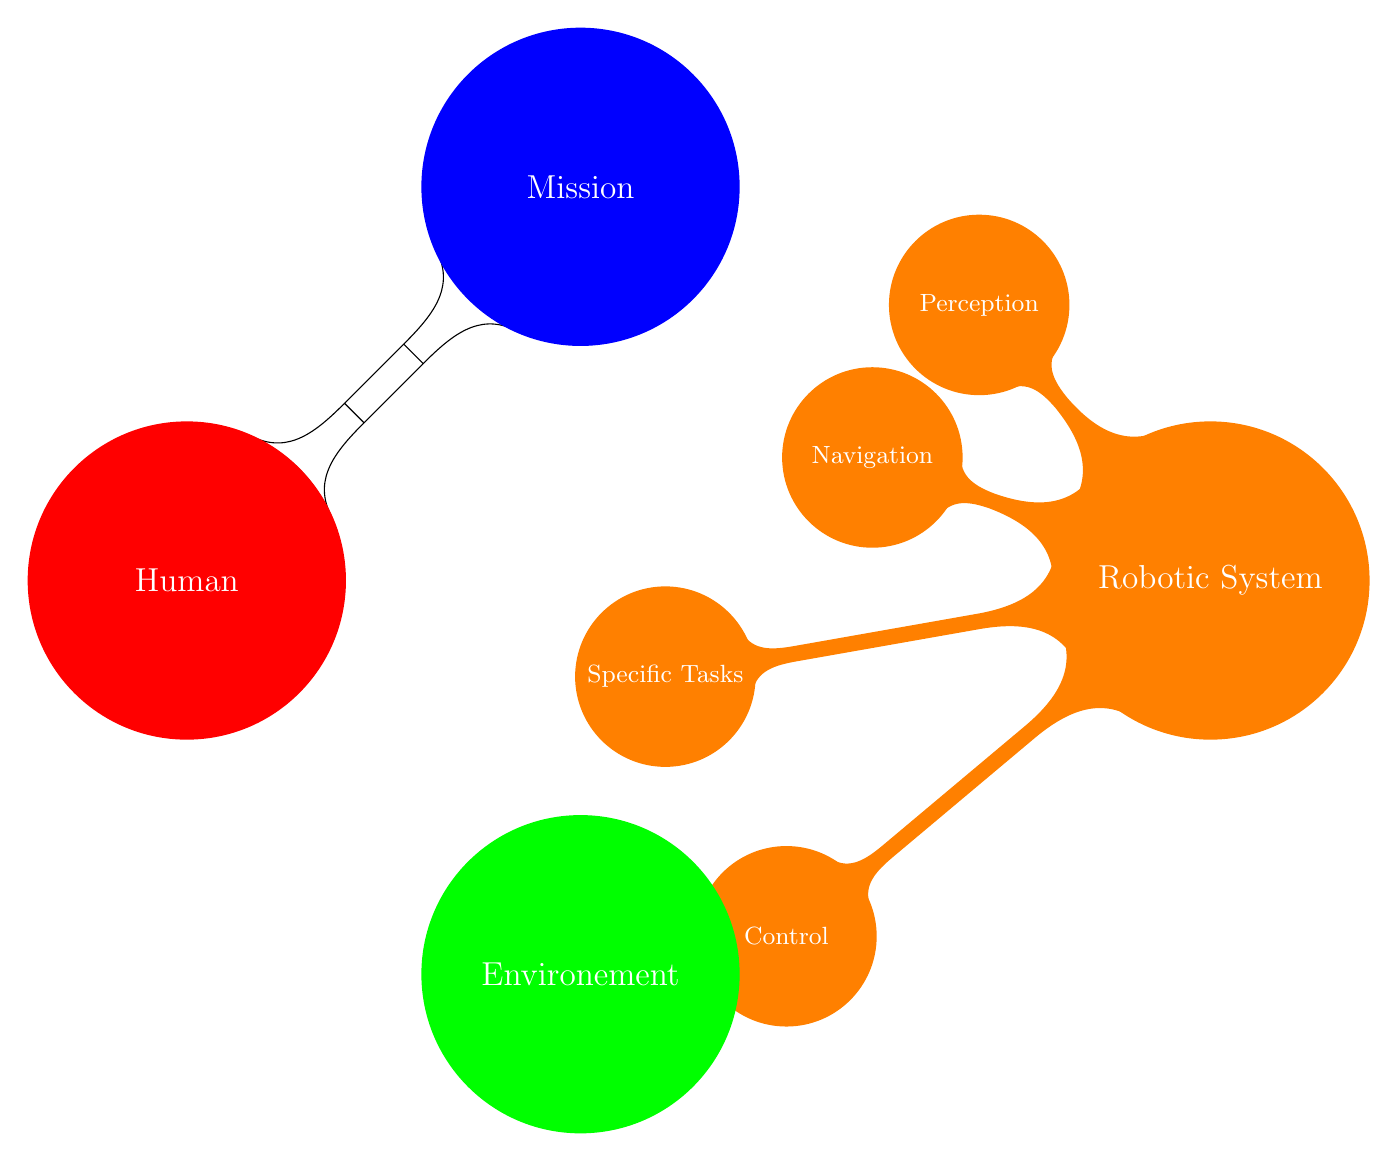
\begin{tikzpicture}[mindmap,
 level 1 concept/.append style={level distance=130,sibling angle=30},
extra concept/.append style={color=blue!50,text=black}]

\begin{scope}[mindmap, concept color=blue,text=white]
 \node [concept] (mis) at (0,0) {Mission};
\end{scope}

\begin{scope}[mindmap, concept color=orange, text=white]
 \node [concept] at (8,-5) {Robotic System}[clockwise from=220]
 child [grow=220, level distance=200] {node [concept] (con) {Control}}
 child [level distance=200] {node [concept] (spe) {Specific Tasks}}
 child {node [concept] (nav) {Navigation}}
 child {node [concept] (per) {Perception}};
\end{scope}

\begin{scope}[mindmap, concept color=red,text=white]
 \node [concept] (hum) at (-5,-5) {Human};
\end{scope}

\begin{scope}[mindmap, concept color=green,text=white]
 \node [concept] at (0,-10) {Environement};
\end{scope}

\begin{pgfonlayer}{background}
 \draw [circle connection bar]
 (mis) edge (hum);
\end{pgfonlayer}

\end{tikzpicture}

\end{document}
